% =====================================================================
% AsymVerify  -  SemEval-2026 Task 6 (CLARITY), Subtask 1
% Gemini beamerposter theme (anishathalye/gemini, MIT), purple, Times,
% A0 portrait. Layout modeled on the Pollice Verso (Wuerzburg) poster:
% tl;dr + Overview, three method columns, full-width architecture,
% two-column results, conclusion. Compile with lualatex.
% Content cross-checked against the CLARITY task paper (2026.semeval-1.449).
% =====================================================================
\PassOptionsToPackage{table}{xcolor}
\documentclass[final]{beamer}
\usepackage[T1]{fontenc}
\usepackage[size=custom,width=91,height=119,scale=1.0]{beamerposter}
\usetheme{gemini}
\usecolortheme{gemini}
\usepackage{graphicx}
\usepackage{booktabs}
\usepackage{amsmath}
\usepackage{tikz}
\usepackage{tcolorbox}
\tcbuselibrary{skins}
\usepackage{fontawesome5}
\usepackage{qrcode}
\usepackage{tabularx}
\usepackage{wrapfig}
\graphicspath{{figures/}{assets/}}
% light rounded content box (reference-style panels)
\newtcolorbox{tbox}[1][]{enhanced, arc=3mm, colback=white, colframe=violetA!55, boxrule=1.1pt,
  left=3mm, right=3mm, top=2.5mm, bottom=2mm, #1}

% ---- Lato + larger body ----
\setmainfont{Lato}
\renewcommand{\familydefault}{\rmdefault}
\setbeamerfont{headline title}{family=\rmfamily,series=\bfseries,size=\huge}
\setbeamerfont{headline author}{family=\rmfamily,series=\bfseries,size=\Large}
\setbeamerfont{headline institute}{family=\rmfamily,size=\large}
\setbeamerfont{block title}{family=\rmfamily,series=\bfseries,size=\huge}
\newcommand{\blockbodysize}{\fontsize{24.4}{28.8}\selectfont}
\setbeamerfont{block body}{family=\rmfamily,size=\blockbodysize}
\setbeamerfont{heading}{family=\rmfamily,series=\bfseries,size=\large}
\setbeamerfont{footline}{family=\rmfamily,size=\large}
\setbeamerfont{headline}{family=\rmfamily}

% ---- geometry: variable-width rows (Wuerzburg-style) ----
\newlength{\sepwidth}\setlength{\sepwidth}{0.025\paperwidth}
\newlength{\tldrW}\setlength{\tldrW}{0.30\paperwidth}
\newlength{\ovW}\setlength{\ovW}{0.620\paperwidth}
\newlength{\triW}\setlength{\triW}{0.30\paperwidth}
\newlength{\halfW}\setlength{\halfW}{0.4625\paperwidth}
\newlength{\fullwidth}\setlength{\fullwidth}{\dimexpr3\triW+2\sepwidth\relax}
\newlength{\archw}\setlength{\archw}{0.545\fullwidth}
\newcommand{\separatorcolumn}{\begin{column}{\sepwidth}\end{column}}

\newcommand{\clCR}{\textbf{\color{passThree}CR}}
\newcommand{\clAMB}{\textbf{\color{purpleBrand}AMB}}
\newcommand{\clCNR}{\textbf{\color{passTwo}CNR}}
\renewcommand{\arraystretch}{1.05}
\newcommand{\archfig}{\IfFileExists{figures/fig_arch.pdf}%
  {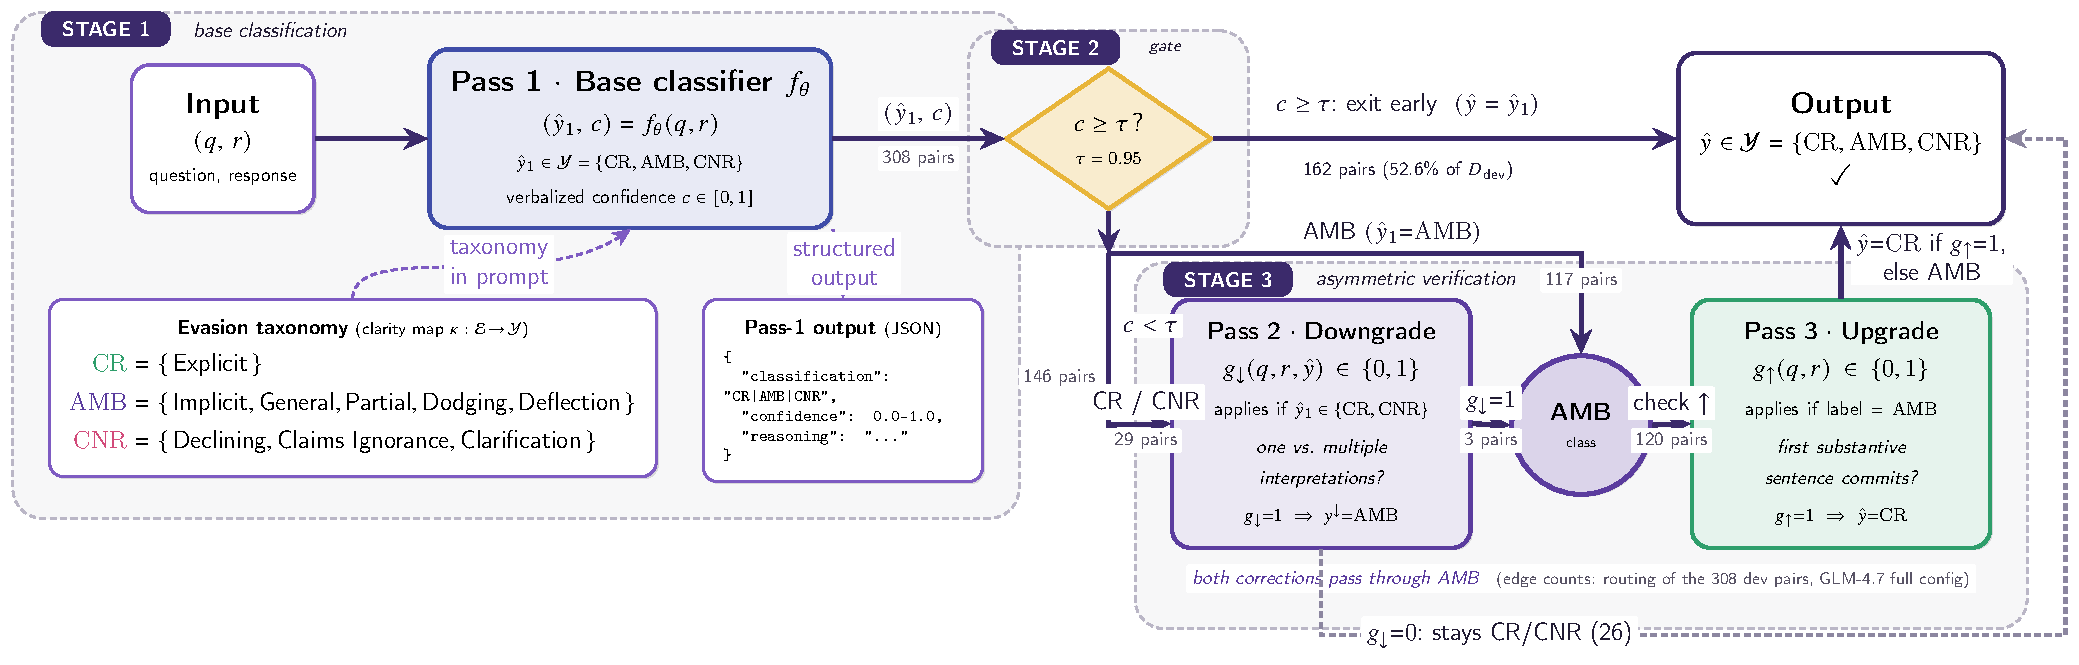
\includegraphics[width=\linewidth]{figures/fig_arch.pdf}}%
  {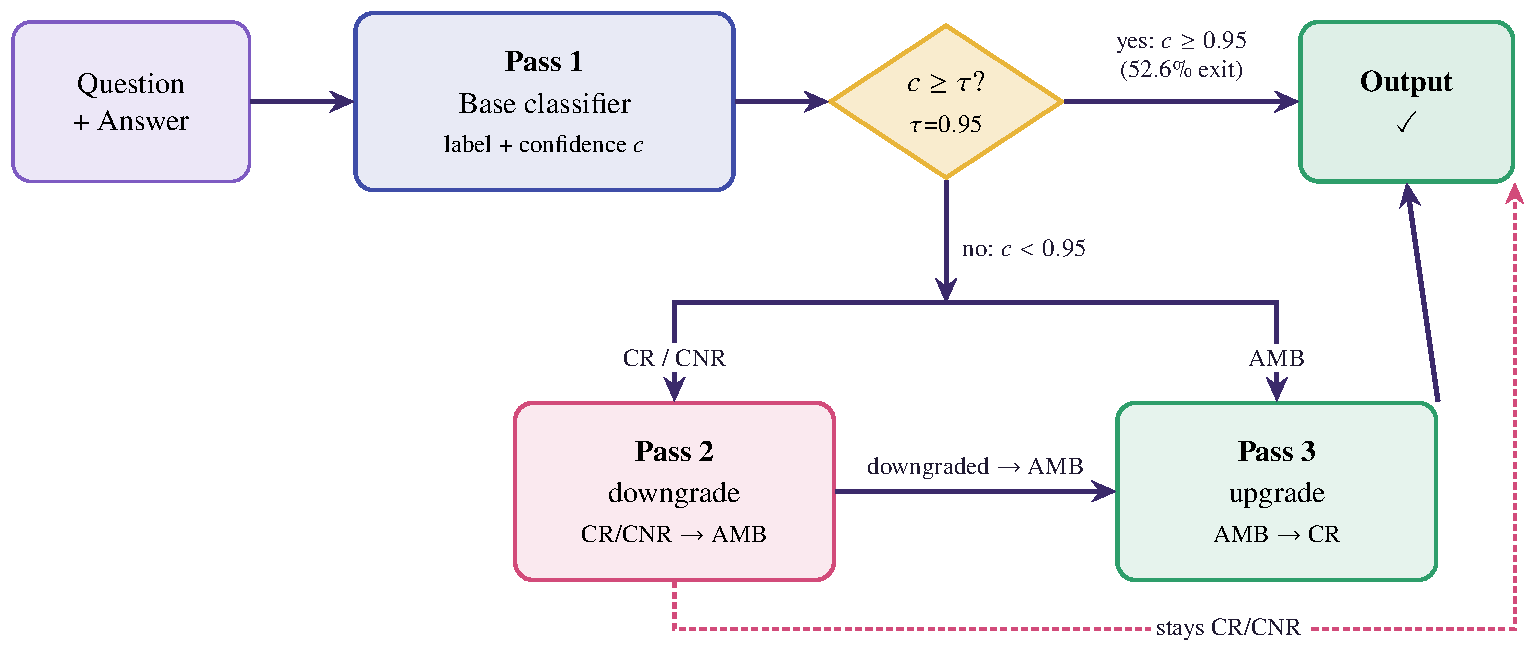
\includegraphics[height=15cm]{figures/fig_cascade.pdf}}}

\title{AsymVerify at SemEval-2026 Task 6:\\Asymmetric Confidence-Gated Verification\\for Political Evasion Detection}
\author{Sebastien Kawada}
\institute{Kaons, Los Angeles, CA, USA \enspace\textbar\enspace CLARITY, Subtask 1 (Clarity-level Classification) \enspace\textbar\enspace sebastien@kaons.com}

% ACL logo recomposed: vector-derived mark (556 ppi) + typeset wordmark,
% replacing the 74 ppi acl-logo.png that pixelated at print size.
\definecolor{aclInk}{HTML}{232A34}
\logoleft{\hspace*{16mm}\vbox{%
  \hbox{
\includegraphics[height=4.4cm]{assets/acl-mark.png}}\vskip 3.5mm
  \hbox{\resizebox{6.5cm}{!}{\textbf{\textcolor{aclInk}{ACL 2026}}}}}\hspace*{-16mm}}
\logoright{\vbox{%
  \hbox{
\includegraphics[height=6.6cm]{assets/kaons-logo.pdf}}\vskip 2.5mm
  \hbox{
\includegraphics[width=6.6cm]{assets/ucla-logo.png}}}}

\footercontent{%
  \faGithub~\texttt{github.com/kaons-research/AsymVerify-ACL} \hfill
  ACL 2026 / SemEval-2026, San Diego \hfill
  \faEnvelope~\texttt{sebastien@kaons.com}}

% =====================================================================
\begin{document}
\begin{frame}[t]

% ============ ROW A: Task Overview + Related Work (narrow left) | credited task figures (right) ============
\begin{columns}[t]
\separatorcolumn
\begin{column}{0.40\paperwidth}
  \begin{block}{Task Overview}
    \begin{itemize}
      \item \textbf{SemEval-2026 Task~6 (CLARITY), Subtask~1}: classify each political
        question--answer pair from U.S.\ presidential interviews by \emph{response clarity} --
        did the speaker commit, regardless of position?
      \item \clCR{} direct commitment; \clAMB{} evasive (vague, partial, topic-shifting);
        \clCNR{} explicit refusal / claim of ignorance.
      \item Ranked by \textbf{Macro F1}: the dev split is 67\% Ambivalent, so majority-class
        accuracy is trivially high while balanced per-class F1 is not.
    \end{itemize}
  \end{block}
  \begin{tbox}[colback=lavender!60, colframe=purpleBrand, boxrule=1.6pt,
               left=4mm, right=4mm, top=2.5mm, bottom=2.5mm]
    {\large\bfseries\color{purpleDeep}Key insight: all roads lead through Ambivalent.}\\[1.5mm]
    CR and CNR are opposite speech acts, almost never confused directly (3\% of errors).
    Mistakes pile up at the two AMB boundaries instead: evasion over-credited as commitment
    (63\%), real commitments dismissed as evasive (29\%). Two boundary-aimed verifiers
    therefore cover $>$92\% of errors -- and a confidence gate fires them only where
    Pass~1 is unsure.
  \end{tbox}
  \begin{block}{Related Work}
    \begin{itemize}
      \item \textbf{Dataset \& taxonomy.} Thomas et al.\ (2024) introduced CLARITY:
        U.S.\ presidential interviews with a CR/AMB/CNR clarity label over a nine-subtype
        evasion typology.
      \item \textbf{Prompted \emph{vs.}\ fine-tuned.} CLARITY recasts long-studied political
        equivocation as supervised classification; LLM prompting beats the fine-tuned
        baseline, and every top-ranked system is prompting-based.
      \item \textbf{Self-verification, selectively.} AsymVerify applies self-correction only
        to low-confidence cases and only toward AMB/CR; verbalized confidence is a routing
        signal, not a calibrated probability.
    \end{itemize}
  \end{block}
\end{column}
\separatorcolumn
\begin{column}{0.52\paperwidth}
  \begin{minipage}[t]{0.41\linewidth}
    \vspace{0.9cm}
    \begin{tbox}[height=8.7cm,valign=center]
      \centering
      {\color{purpleBrand}\textbf{Data \& metric}}\\[2mm]
      \small
      \begin{tabular}{@{}lrrrr@{}}
        \toprule
        \textbf{Split} & \textbf{Pairs} & \textbf{\% AMB} & \textbf{\% CR} & \textbf{\% CNR} \\
        \midrule
        Train & 3{,}448 & 59\% & 31\% & 10\% \\
        Dev & 308 & 67\% & 26\% & 8\% \\
        Eval & 237 & \multicolumn{3}{c}{\textit{hidden}} \\
        \bottomrule
      \end{tabular}\\[3mm]
      $\mathrm{Macro\,F1}{=}\tfrac13\big(\mathrm{F1}_{\mathrm{CR}}\!+\!\mathrm{F1}_{\mathrm{AMB}}\!+\!\mathrm{F1}_{\mathrm{CNR}}\big)$\\[2mm]
      {\footnotesize\color{purpleBrand}Imbalanced, AMB-dominant}
    \end{tbox}
    \vspace{4mm}
    \begin{tbox}[height=8.7cm,valign=center]
      \centering
      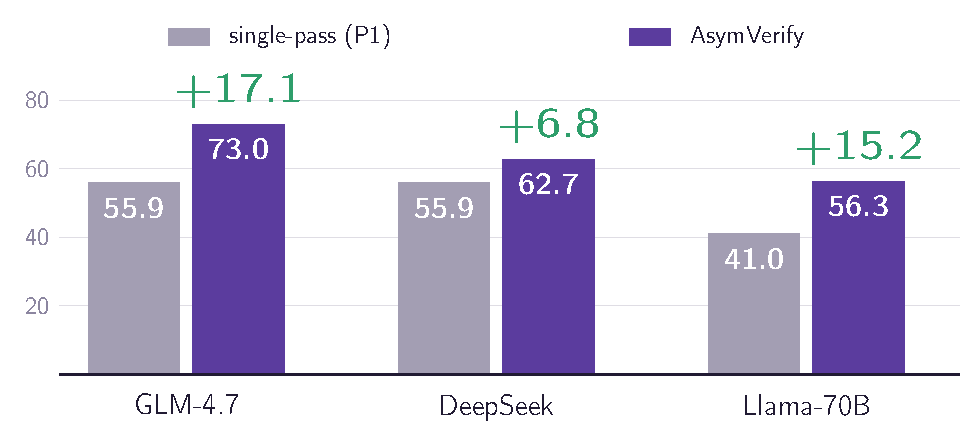
\includegraphics[height=6.1cm]{figures/fig_uplift.pdf}
      \\[1mm]{\footnotesize\color{purpleBrand}\textbf{AsymVerify uplift over single-pass baseline}\\ (Macro F1, $D_{\mathrm{dev}}$; best variant per model)}
    \end{tbox}
  \end{minipage}\hfill
  \begin{minipage}[t]{0.56\linewidth}
    \vspace{0.9cm}
    \begin{tbox}
      \centering
      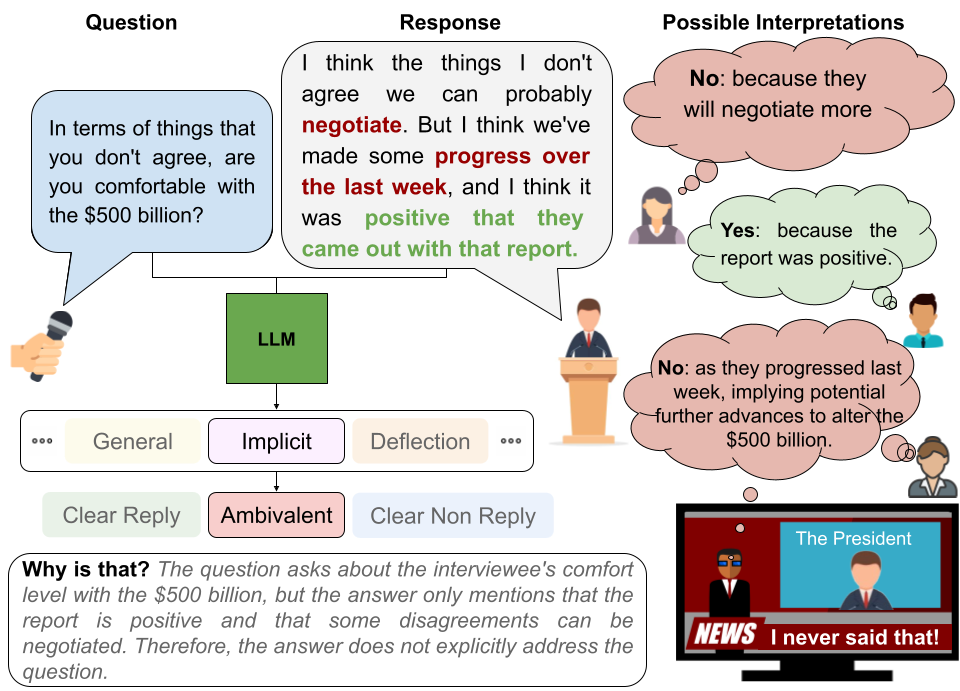
\includegraphics[width=\linewidth]{assets/task_fig1.png}
      \\[1mm]{\footnotesize\color{purpleBrand}\textbf{A classified CLARITY example}\\ (Thomas et al., 2024, arXiv:2409.13879)}
    \end{tbox}
  \end{minipage}
  \par\vspace{0.5mm}
  {\large\color{purpleBrand}\textbf{How AsymVerify works, in four panels}}\par\vspace{1mm}
  \includegraphics[width=\linewidth]{assets/goose.png}
\end{column}
\separatorcolumn
\end{columns}

% ============ ROW C: full-width architecture ============
\begin{columns}[t]
\separatorcolumn
\begin{column}{\fullwidth}
  \begin{minipage}[c]{0.565\linewidth}
    \centering
    \begin{tikzpicture}[remember picture]
      \node[inner sep=0] (archnode) {\phantom{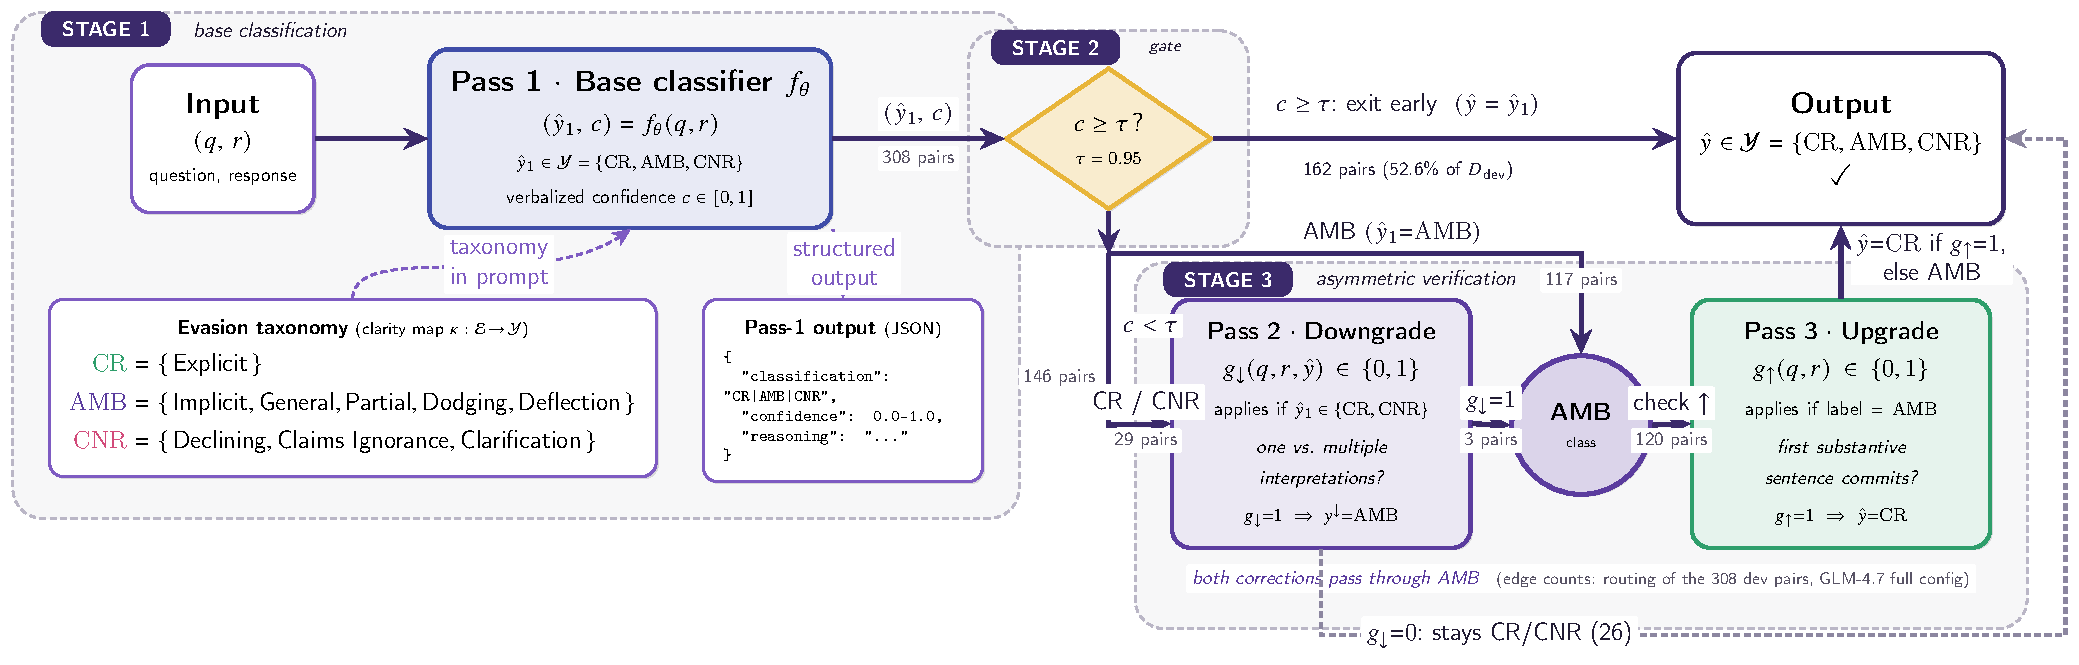
\includegraphics[width=\archw]{figures/fig_arch.pdf}}};
    \end{tikzpicture}
  \end{minipage}\hfill
  \begin{minipage}[c]{0.405\linewidth}
      \begin{beamercolorbox}[colsep*=0ex,dp=1.5ex,center]{block title}
        \usebeamerfont{block title}System Architecture
        \vskip-1.25ex
        \begin{beamercolorbox}[colsep=0.025ex]{block separator}\end{beamercolorbox}
      \end{beamercolorbox}
      \vspace{2mm}
      \textbf{Stage 1 (classify):} one LLM pass $f_\theta$ returns structured JSON:
      a label $\hat y_1$ plus verbalized confidence $c$, the nine-subtype taxonomy
      in-prompt as a clarity map $\kappa:\mathcal E\!\to\!\mathcal Y$.
      \par\medskip
      \textbf{Stage 2 (gate):} if $c\ge\tau{=}0.95$, exit immediately ($\hat y{=}\hat y_1$).
      52.6\% of dev pairs exit here, and this slice is also the most accurate (80.9\%).
      \par\medskip
      \textbf{Stage 3 (verify):} low-confidence CR/CNR predictions get the downgrade
      check $g_\downarrow$; whatever is labeled AMB afterwards (117 direct $+$ 3
      downgraded) gets the upgrade check $g_\uparrow$; either direction alone recovers
      most of the gain.
  \end{minipage}
\end{column}
\separatorcolumn
\end{columns}
\vspace{-1.65cm}

% ============ ROW D: two-column Results / Analysis ============
\begin{columns}[t]
\separatorcolumn
\begin{column}{\halfW}
  \begin{block}{Results}
    {\itshape Submission GPT-5.2 (reasoning\_effort=high); development on GLM-4.7,
    DeepSeek-V3.2, Llama-3.3-70B; $\tau{=}0.95$; 1{,}000-sample paired bootstrap.}
    \par\medskip
    \begin{minipage}[t]{0.52\linewidth}
      \vspace{0pt}
      \textbf{Official leaderboard.} Of 124 registered teams (946 submitted runs), 41
      reached the ranked leaderboard. AsymVerify scored \textbf{0.85} Macro F1 on eval
      ($D_{\mathrm{eval}}$, $n{=}237$): \textbf{2nd of 41}, one of only seven teams to
      match or beat the strong 0.82 fine-tuned baseline. The winner reached Subtask~1
      \emph{indirectly} (via the fine-grained evasion subtask); AsymVerify classifies
      clarity directly, yet lands within 0.04 Macro F1 of it.
      \par\medskip
      \textbf{Why the task is hard.} Fleiss $\kappa$ measures agreement between
      independent annotators, corrected for chance ($1.0$ = unanimity). Humans separate
      CR from CNR almost perfectly ($\kappa{=}0.97$) but falter once Ambivalent is
      involved ($\kappa{=}0.65$--$0.71$): the gold labels are noisy exactly at the AMB
      boundaries, an effective performance ceiling that AsymVerify's 0.85 approaches.
    \end{minipage}\hfill
    \begin{minipage}[t]{0.44\linewidth}
      \vspace{0pt}\centering\fontsize{20}{23.5}\selectfont
      \begin{tabular}{@{}clc@{}}
        \toprule
        \textbf{Rank} & \textbf{Team} & \textbf{Macro-F1} \\
        \midrule
        1 & TeleAI & 0.89 \\
        \rowcolor{lavender}\textbf{2} & \textbf{AsymVerify (ours)} & \textbf{0.85} \\
        3 & CSE-UOI & 0.85 \\
        4 & Rasende Rakete & 0.83 \\
        5 & Evaluators & 0.83 \\
        6 & YNU-HPCC & 0.83 \\
        7 & moswisarut & 0.82 \\
        \midrule
        \multicolumn{2}{@{}l}{\textit{Baseline (fine-tuned Llama-70B)}} & \textit{0.82} \\
        \midrule
        \color{slateA}8 & \color{slateA}tahamunawar & \color{slateA}0.81 \\
        \color{slateA}9 & \color{slateA}CLaC @ CLARITY & \color{slateA}0.80 \\
        \color{slateA}10 & \color{slateA}SpinDetector & \color{slateA}0.80 \\
        \bottomrule
      \end{tabular}
    \end{minipage}
    \par\medskip
    \begin{minipage}[t]{0.52\linewidth}
      \vspace{0pt}
      \textbf{Ablation} ($D_{\mathrm{dev}}$, GLM-4.7). Each verifier adds ${\sim}$+15 Macro F1;
      together \textbf{+17.1} at 1.48 calls/example, half of running all passes. P1+P2 and P1+P3
      are statistically indistinguishable (CI $[-5.9,5.9]$) since both correct
      \emph{through} AMB; the P2/P3 columns count verifier activations.
    \end{minipage}\hfill
    \begin{minipage}[t]{0.44\linewidth}
      \vspace{0pt}\centering\fontsize{20}{23.5}\selectfont
      \begin{tabular}{@{}lrrrrr@{}}
        \toprule
        \textbf{Configuration} & \textbf{Macro} & \textbf{Acc.} & \textbf{Calls} & \textbf{P2} & \textbf{P3} \\
        \midrule
        P1 (single pass) & 55.9 & 77.6 & 1.00 & 0 & 0 \\
        P1\,+\,P2 & 70.9 & 76.0 & 1.15 & 45 & 0 \\
        P1\,+\,P3 & 70.8 & 72.1 & 1.33 & 0 & 102 \\
        \rowcolor{lavender}\textbf{P1\,+\,P2\,+\,P3} & \textbf{73.0} & \textbf{75.3} & 1.48 & 29 & 120 \\
        \bottomrule
      \end{tabular}
    \end{minipage}
  \end{block}

  \begin{block}{Verification in Action}
    \textbf{1. Buried commitment (Pass-3 save).} \textbf{Q.}~``...building the 700 miles of
    fence?'' \textbf{A.}~``\textbf{Yes}, we're going to do both, Joe\,\ldots'' Pass~1 (confidence 0.85) says
    \textbf{Ambivalent}, distracted by the later qualifier; Pass~3 anchors on ``Yes'' and
    restores \textbf{Clear Reply} (gold: CR).
    \par\medskip
    \textbf{2. Parse-failure recovery.} When Pass~1 returns no valid JSON and defaults to AMB at
    confidence 0.0, the low-confidence route still reaches Pass~3, which reads a flat
    ``\textbf{Absolutely.} No ands, ifs, or buts,'' and restores \textbf{Clear Reply}; the gate
    degrades gracefully on malformed output.
  \end{block}
\end{column}
\separatorcolumn
\begin{column}{\halfW}
  \begin{block}{Analysis}
    \begin{minipage}[t]{0.53\linewidth}
      \vspace{0pt}
      \textbf{It is the mechanism, not the model.} The Pass-3 upgrade improves \emph{every}
      backend (+6.8 to +15.2 Macro F1), so the gain is the asymmetric design, not one lucky
      model. Downgrade is more model-sensitive (over-corrects DeepSeek/Llama). Per-class: AMB
      most transferable (79.8--83.1), CNR most model-dependent (34.5--75.0), CR intermediate
      (51.2--62.9).
    \end{minipage}\hfill
    \begin{minipage}[t]{0.44\linewidth}
      \vspace{0pt}\centering\fontsize{20}{23.5}\selectfont
      \setlength{\tabcolsep}{4.5pt}%
      \begin{tabular}{@{}llrrrrr@{}}
        \toprule
        \textbf{Model} & \textbf{Cfg} & \textbf{Mac} & \textbf{$\Delta$} & \textbf{CR} & \textbf{AMB} & \textbf{CNR} \\
        \midrule
        GLM-4.7 & \textbf{full} & \textbf{73.0} & \color{passThree}+17.1 & 62.9 & 81.0 & 75.0 \\
        DeepSeek & \textbf{+P3} & \textbf{62.7} & \color{passThree}+6.8 & 57.0 & 79.8 & 51.4 \\
        Llama-70B & \textbf{+P3} & \textbf{56.3} & \color{passThree}+15.2 & 51.2 & 83.1 & 34.5 \\
        \bottomrule
      \end{tabular}
    \end{minipage}
    \par\medskip
    \textbf{Where the errors are.} Of 76 dev errors, \textbf{63.2\%} lie on the downgrade
    $(\text{CR/CNR}\!\to\!\text{AMB})$ boundary and \textbf{28.9\%} on the upgrade
    $(\text{AMB}\!\to\!\text{CR})$ boundary; only \textbf{7.9\%} outside, so two verifiers address
    $>$92\%. A paired bootstrap confirms the Llama $\text{P1}\!\to\!\text{P1+P3}$ lift is
    significant (+15.2, CI $[7.5,23.1]$).
    \par\medskip
    \textbf{Cost.} Gating routes 52.6\% to output after Pass~1: \textbf{457 calls vs 924}, a
    50.5\% cut. \textbf{Why not embeddings?} 3{,}756 Gemini embeddings (3{,}072-d) under UMAP
    give silhouette 0.001; clarity lives in pragmatic cues embeddings miss.
  \end{block}
  \begin{block}{Why the Gate Works}
    \begin{minipage}[t]{0.52\linewidth}
      \vspace{0pt}
      Verbalized confidence is over-confident but cleanly \emph{ranks} difficulty: both accuracy
      and Macro F1 rise from the lowest to the highest bin, Macro F1 far more sharply
      (\textbf{25.6}$\to$\textbf{78.8} vs 62.5$\to$80.9). The $c\!\ge\!0.95$ early-exit set is
      both the largest and the best, so verifier calls are spent only where they can change the
      answer, below $\tau$.
    \end{minipage}\hfill
    \begin{minipage}[t]{0.45\linewidth}
      \vspace{0pt}\centering\fontsize{20}{23.5}\selectfont
      \begin{tabular}{@{}lrrr@{}}
        \toprule
        \textbf{Confidence bin} & \textbf{n} & \textbf{Acc.} & \textbf{Macro} \\
        \midrule
        $c<0.70$ & 16 & 62.5\% & 25.6 \\
        \color{slateA}$0.70\text{--}0.80$ & \color{slateA}2 & \color{slateA}50.0\% & \color{slateA}33.3 \\
        $0.80\text{--}0.90$ & 34 & 76.5\% & 69.8 \\
        $0.90\text{--}0.95$ & 94 & 78.7\% & 69.2 \\
        \rowcolor{lavender}$c\ge0.95$ & 162 & \textbf{80.9\%} & \textbf{78.8} \\
        \bottomrule
      \end{tabular}
    \end{minipage}
    \par\smallskip
    \textbf{Optional lexical prefilter.} A cheap deterministic filter: fire Pass 3 only when the
    first sentence opens with a commitment cue (cutting P3 calls and false upgrades sharply):
    \par\vspace{-3pt}
    \begin{minipage}[t]{0.44\linewidth}
      \vspace{0pt}
      \begin{itemize}\setlength\itemsep{1pt}\setlength\topsep{0pt}\setlength\partopsep{0pt}
        \item \emph{No} $+$ short declarative
        \item \emph{Because} (causal explanation)
        \item \emph{That is} / \emph{That's} (assertion)
        \item \emph{No, I don't see} (stance)
      \end{itemize}
    \end{minipage}\hfill
    \begin{minipage}[t]{0.52\linewidth}
      \vspace{0pt}\centering\fontsize{20}{23.5}\selectfont
      \begin{tabular}{@{}lrrrr@{}}
        \toprule
        \textbf{Variant} & \textbf{Macro F1} & \textbf{Acc.} & \textbf{P3 calls} & \textbf{False up.} \\
        \midrule
        No prefilter & 73.0 & 75.3 & 120 & 19 \\
        \rowcolor{lavender}$+$ lexical prefilter & \textbf{74.7} & \textbf{78.9} & \textbf{3} & \textbf{0} \\
        \bottomrule
      \end{tabular}
    \end{minipage}
  \end{block}
\end{column}
\separatorcolumn
\end{columns}

% ============ ROW E: full-width Conclusion and Future Directions ============
\begin{columns}[t]
\separatorcolumn
\begin{column}{\fullwidth}
  \begin{block}{Conclusion and Future Directions}
    \begin{minipage}[t]{0.66\linewidth}
      \vspace{0pt}
      Errors concentrate at the Ambivalent boundary and both corrections route through it,
      so selective asymmetric verification recovers most errors at low cost. AsymVerify placed
      \textbf{2nd of 41 teams} (0.85 Macro F1), backend-agnostic across GLM-4.7,
      DeepSeek-V3.2, and Llama-3.3-70B.
      \begin{itemize}
        \item \textbf{Per-model gating:} downgrade verification over-corrects some backends; a
          learned per-model threshold should recover the lost Clear Non-Reply precision.
        \item \textbf{Calibrated confidence:} a calibrated gate signal would route borderline
          cases better and cut calls further.
        \item \textbf{Beyond English:} the mechanism is language-agnostic and worth testing on
          multilingual political discourse. Labels describe response clarity, not truth or intent.
      \end{itemize}
    \end{minipage}\hfill
    \begin{minipage}[t]{0.30\linewidth}
      \centering\vspace{0pt}
      \begin{minipage}[t]{0.47\linewidth}
        \centering\vspace{0pt}
        \begin{tikzpicture}
          \node[draw=purpleDeep, line width=1.6pt, densely dashed, rounded corners=5mm,
                inner sep=2.5mm, fill=white]
            {\qrcode[height=4.3cm]{https://github.com/kaons-research/AsymVerify-ACL}};
        \end{tikzpicture}\\[1mm]
        \textbf{Code, prompts \& paper}\\[0.5mm]
        {\scriptsize\texttt{github.com/kaons-research/}}\\
        {\scriptsize\texttt{AsymVerify-ACL}}
      \end{minipage}\hfill
      \begin{minipage}[t]{0.47\linewidth}
        \centering\vspace{0pt}
        \begin{tikzpicture}
          \node[draw=purpleDeep, line width=1.6pt, densely dashed, rounded corners=5mm,
                inner sep=2.5mm, fill=white]
            {\qrcode[height=4.3cm]{https://www.linkedin.com/in/sebastienkawada/}};
        \end{tikzpicture}\\[1mm]
        \textbf{Connect on LinkedIn}\\[0.5mm]
        {\scriptsize\texttt{linkedin.com/in/}}\\
        {\scriptsize\texttt{sebastienkawada}}
      \end{minipage}
    \end{minipage}
  \end{block}
\end{column}
\separatorcolumn
\end{columns}

% Draw the architecture diagram last so it renders on top of any overlapping section.
\begin{tikzpicture}[remember picture, overlay]
  \node[inner sep=0] at (archnode) {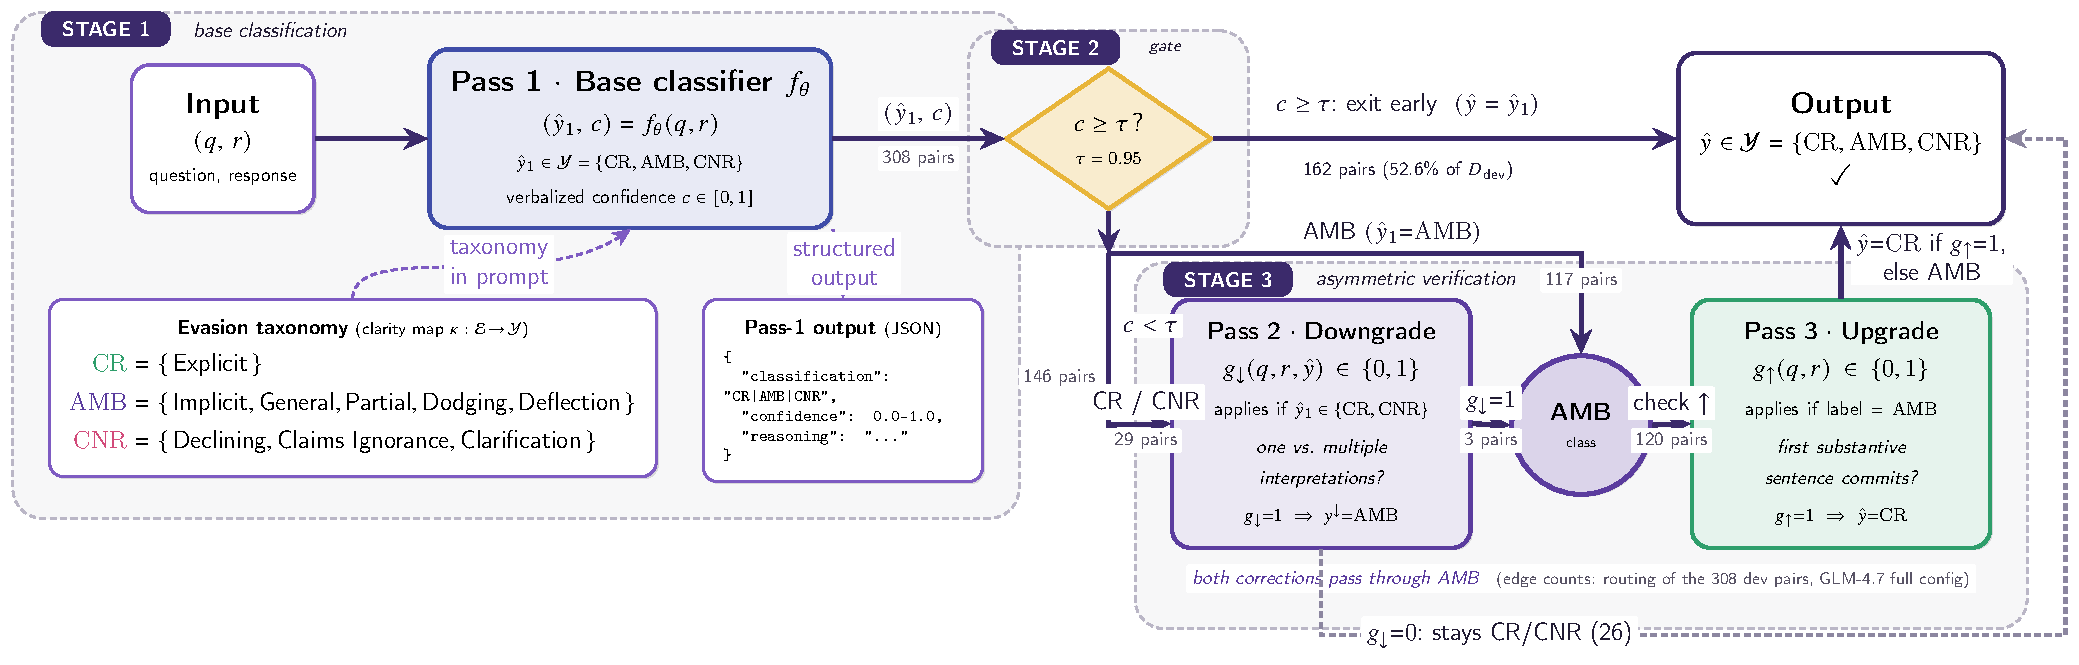
\includegraphics[width=\archw]{figures/fig_arch.pdf}};
\end{tikzpicture}
\end{frame}
\end{document}
